\documentclass[11pt]{article}

\usepackage[a4paper,margin=0.6in]{geometry}
\usepackage{amsmath,amssymb}
\usepackage{tikz}
\usepackage{tcolorbox}
\usepackage{multicol}
\usepackage{xcolor}

\pagestyle{empty}

\begin{document}

\begin{center}
    {\Huge \textbf{Algebra 1 -- Transformations Worksheet}}
\end{center}

\vspace{0.3cm}

%=========================================================
% SECTION A
%=========================================================

\begin{tcolorbox}[colback=blue!5,colframe=blue,title=\Large A. Warm Up -- Directions from a Point]

\textbf{Find the new point after moving in the given direction.}

\vspace{0.3cm}

\begin{multicols}{2}

\textbf{1. Point $P(2,1)$}

\begin{itemize}
    \item Left 1: \underline{\hspace{2cm}}
    \item Right 2: \underline{\hspace{2cm}}
    \item Up 3: \underline{\hspace{2cm}}
    \item Down 4: \underline{\hspace{2cm}}
\end{itemize}

\begin{center}
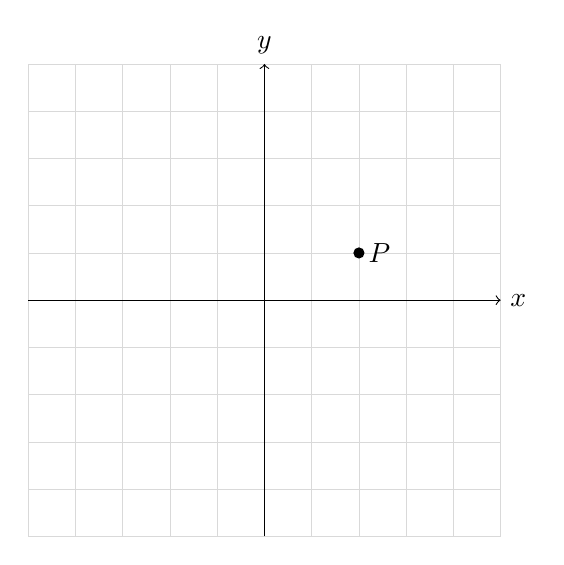
\begin{tikzpicture}[scale=0.6]
    \draw[step=1cm,gray!30,very thin] (-5,-5) grid (5,5);
    \draw[->] (-5,0)--(5,0) node[right]{$x$};
    \draw[->] (0,-5)--(0,5) node[above]{$y$};
    \filldraw (2,1) circle (3pt) node[right]{$P$};
\end{tikzpicture}
\end{center}

\columnbreak

\textbf{2. Point $P(-3,2)$}

\begin{itemize}
    \item Left 1: \underline{\hspace{2cm}}
    \item Right 2: \underline{\hspace{2cm}}
    \item Up 3: \underline{\hspace{2cm}}
    \item Down 4: \underline{\hspace{2cm}}
\end{itemize}

\begin{center}
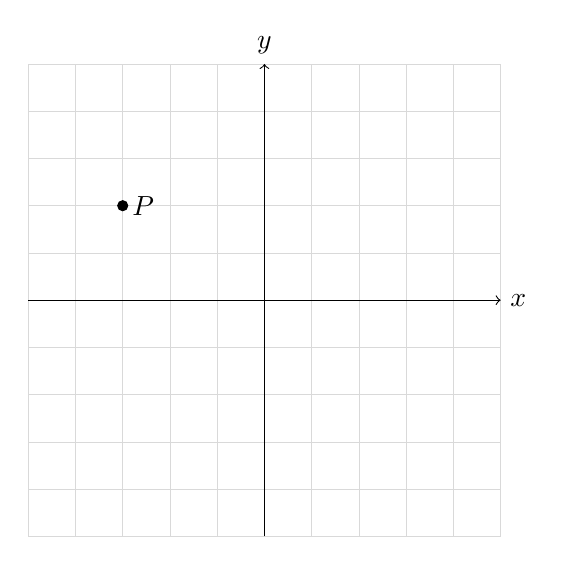
\begin{tikzpicture}[scale=0.6]
    \draw[step=1cm,gray!30,very thin] (-5,-5) grid (5,5);
    \draw[->] (-5,0)--(5,0) node[right]{$x$};
    \draw[->] (0,-5)--(0,5) node[above]{$y$};
    \filldraw (-3,2) circle (3pt) node[right]{$P$};
\end{tikzpicture}
\end{center}

\end{multicols}

\vspace{0.3cm}

\textbf{Direction Rules}

\[
\text{Left 1: } (x-1,y)
\]

\[
\text{Right 2: } (x+2,y)
\]

\[
\text{Up 3: } (x,y+3)
\]

\[
\text{Down 4: } (x,y-4)
\]

\end{tcolorbox}

\vspace{0.5cm}

%=========================================================
% SECTION B
%=========================================================

\begin{tcolorbox}[colback=green!5,colframe=green!60!black,title=\Large B. Stretch / Shrink (Dilations)]

\textbf{Graph the image after the transformation.}

\vspace{0.4cm}

\begin{multicols}{3}

\textbf{1. Horizontal Stretch by factor of 2}

\[
(x,y)\rightarrow(2x,y)
\]

\begin{center}
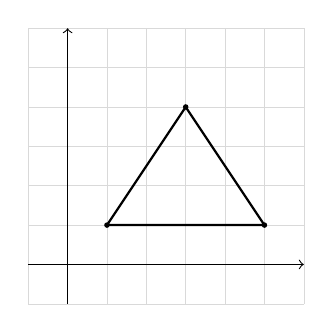
\begin{tikzpicture}[scale=0.5]
    \draw[step=1cm,gray!30,very thin] (-1,-1) grid (6,6);
    \draw[->] (-1,0)--(6,0);
    \draw[->] (0,-1)--(0,6);

    \draw[thick]
    (1,1)--(3,4)--(5,1)--cycle;

    \fill (1,1) circle (2pt);
    \fill (3,4) circle (2pt);
    \fill (5,1) circle (2pt);
\end{tikzpicture}
\end{center}

\columnbreak

\textbf{2. Horizontal Shrink by factor of $\frac12$}

\[
(x,y)\rightarrow\left(\frac12x,y\right)
\]

\begin{center}
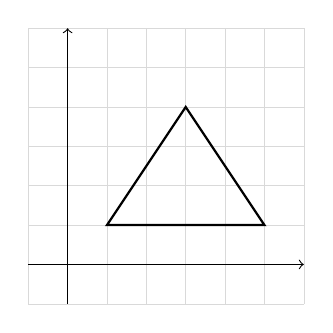
\begin{tikzpicture}[scale=0.5]
    \draw[step=1cm,gray!30,very thin] (-1,-1) grid (6,6);
    \draw[->] (-1,0)--(6,0);
    \draw[->] (0,-1)--(0,6);

    \draw[thick]
    (1,1)--(3,4)--(5,1)--cycle;
\end{tikzpicture}
\end{center}

\columnbreak

\textbf{3. Vertical Stretch by factor of 3}

\[
(x,y)\rightarrow(x,3y)
\]

\begin{center}
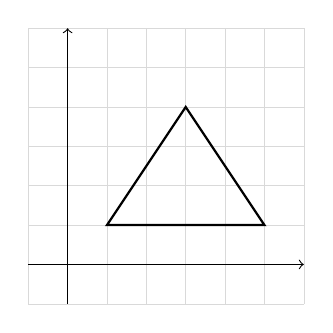
\begin{tikzpicture}[scale=0.5]
    \draw[step=1cm,gray!30,very thin] (-1,-1) grid (6,6);
    \draw[->] (-1,0)--(6,0);
    \draw[->] (0,-1)--(0,6);

    \draw[thick]
    (1,1)--(3,4)--(5,1)--cycle;
\end{tikzpicture}
\end{center}

\end{multicols}

\end{tcolorbox}

\vspace{0.5cm}

%=========================================================
% SECTION C
%=========================================================

\begin{tcolorbox}[colback=purple!5,colframe=purple,title=\Large C. Reflections]

\textbf{Graph the reflected image.}

\vspace{0.3cm}

\begin{multicols}{2}

\textbf{1. Reflect over the $x$-axis}

\[
(x,y)\rightarrow(x,-y)
\]

\begin{center}
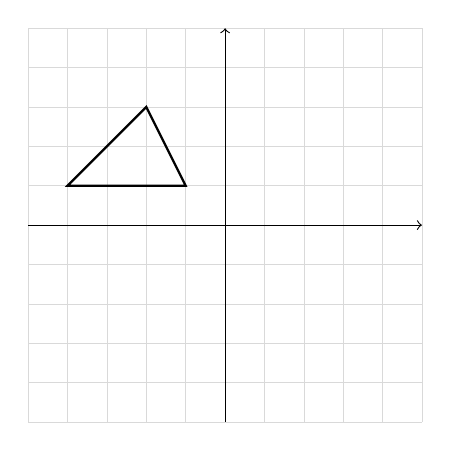
\begin{tikzpicture}[scale=0.5]
    \draw[step=1cm,gray!30,very thin] (-5,-5) grid (5,5);
    \draw[->] (-5,0)--(5,0);
    \draw[->] (0,-5)--(0,5);

    \draw[thick]
    (-4,1)--(-2,3)--(-1,1)--cycle;
\end{tikzpicture}
\end{center}

\columnbreak

\textbf{2. Reflect over the $y$-axis}

\[
(x,y)\rightarrow(-x,y)
\]

\begin{center}
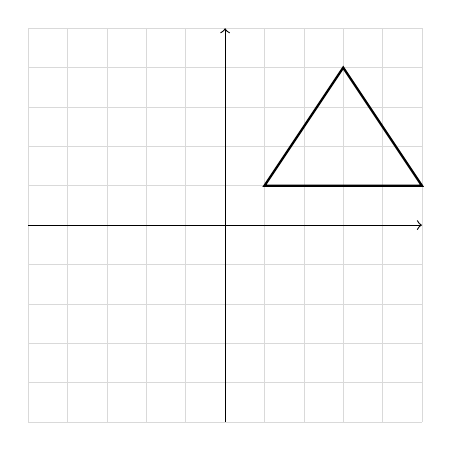
\begin{tikzpicture}[scale=0.5]
    \draw[step=1cm,gray!30,very thin] (-5,-5) grid (5,5);
    \draw[->] (-5,0)--(5,0);
    \draw[->] (0,-5)--(0,5);

    \draw[thick]
    (1,1)--(3,4)--(5,1)--cycle;
\end{tikzpicture}
\end{center}

\end{multicols}

\vspace{0.4cm}

\textbf{Reflection Rules}

\[
\text{Over }x\text{-axis}: (x,y)\rightarrow(x,-y)
\]

\[
\text{Over }y\text{-axis}: (x,y)\rightarrow(-x,y)
\]

\[
\text{Over }y=x: (x,y)\rightarrow(y,x)
\]

\[
\text{Over }y=-x: (x,y)\rightarrow(-y,-x)
\]

\end{tcolorbox}

\vspace{0.5cm}

%=========================================================
% VISUAL GUIDE
%=========================================================

\begin{tcolorbox}[colback=orange!5,colframe=orange,title=\Large Visual Summary]

\begin{itemize}
    \item \textbf{Translations} move a figure.
    \item \textbf{Dilations} change size.
    \item \textbf{Reflections} flip a figure.
    \item Shapes keep the same structure after transformations.
\end{itemize}

\vspace{0.2cm}

\begin{center}
\Large
Practice Daily to Build Transformation Intuition!
\end{center}

\end{tcolorbox}

\end{document}